\projectname~(\projectmeaning) is our realization of the techniques described in
\S\ref{sec:approach}. \projectname~is implemented in roughly 10,000 lines of Python in
addition to the Hassel network invariant checking library~\cite{hsa}. We have
made the code
for \projectname~publicly available.\footnote{URL omitted due to anonymity requirements}
To date, three industrial SDN companies have expressed interest in adopting it.

In the rest of this section, we highlight salient points of \projectname's
design, and illustrate a workflow for users of \projectname.

We show the input types supported by \projectname~in Table~\ref{tab:inputs}.
Our software switches notify controllers about link, switch, and host migration events
by sending OpenFlow messages~\cite{openflow}.
Although the software switches do support packet forwarding, we
have not focused on simulating high-throughput dataplane behavior.
% We hope to support policy changes in the future (Quantum)

\begin{table}
\centering
\begin{tabular}{|l|l|}
\hline
Link failure & Link recovery \\
\hline
Switch failure & Switch recovery \\
\hline
Control server failure & Control server recovery \\
\hline
Dataplane packet injection & Dataplane packet drop \\
\hline
Dataplane packet delay & Dataplane packet permit \\
\hline
Control message delay & Host migration \\
\hline
\end{tabular}
\caption{Input types supported by \projectname}
\label{tab:inputs}
\end{table}

We designed \projectname~to be as resilient to non-determinism as is
practically feasible, while avoiding modifications to control software whenever possible.
When sending data over multiple sockets, the operating system exhibits
non-determinism in the order it schedules the socket I/O operations.
\projectname~optionally ensures a deterministic order of messages
by multiplexing all sockets in the controller process
onto a single true socket.\footnote{Alternatively, we could employ a
mutex~\cite{lin2009towards}.}
\projectname~currently overrides socket functionality within the control
software itself.\footnote{Only supported for POX at the moment.}
In the future we plan to implement deterministic message ordering without code modifications by
loading a shim layer on top of
libc (similar to liblog~\cite{Geels:2006:RDD:1267359.1267386}).

\projectname~needs visibility into the control software's internal state
changes to reliably reproduce the system execution. We achieve this by
making a
small change to the control software's logging library\footnote{Only supported
for POX and Floodlight at the moment.}: whenever a control process executes a log
statement, we notify \projectname~that a new state transition
is about to occur, and optionally block the process. \projectname~then sends
an acknowledgment to unblock the controller after logging the state change. If blocking was enabled
during recording, we force the control software to block at internal state
transition points again during replay
until \projectname~gives explicit acknowledgment.

Routing the {\tt gettimeofday()} syscall
through \projectname~makes replay more resilient to alterations in execution
speeds.\footnote{When the pruned trace differs from the original, we make a
best-effort guess at what the return values of these calls should be. For example,
if the altered execution invokes {\tt gettimeofday()} more times than we recorded
in the initial run, we interpolate the time values of neighboring events}
As an added benefit, overriding {\tt gettimeofday()} allows us to `compress'
runtime in some cases (similar to time-warped emulation~\cite{Gupta06toinfinity}).

If the control software under test utilizes random number generators, we
attempt to manually replace any such functionality with deterministic
algorithms if possible. Our current implementation does not account other sources of non-determinism,
such as asynchronous signals,
or interruptable instructions (\eg~x86's block memory
instructions~\cite{Dunlap:2002:REI:844128.844148}).

\colin{
Need to do a better job of discussing how we stop controllers from getting
ahead of eachother. How do we interpose on intra-controller communication?
(as shown in one of our diagrams)
How do we ensure the same scheduling order of controller processes? (see
Section 4.5 of ReVirt). We observe that the controllers do not use any shared
memory communication.}

Developers and operators can use \projectname~in a number of ways. Here we
illustrate a general workflow.

\subsection{Bug Exploration}
\label{subsec:exploration}

Use of \projectname~begins with bug exploration.
\projectname~itself is well-suited for finding input traces that trigger bugs:
it readily simulates common network input events, and ships with a suite of invariant checking
algorithms~\cite{hsa}. With complete control over event orderings, \projectname~is
especially useful for exploring corner cases.
Along these lines, Amin Vahdat
has testified to the value of Google's SDN network simulator~\cite{vadhat}:
\begin{quote}
``One of the key benefits we have is a very nice emulation and
simulation environment where the exact same control software that would be
running on servers might be controlling a combination of real and emulated
switching devices. And then we can inject a number of failure scenarios under
controlled circumstances to really accelerate our test work.''
\end{quote}
\colin{Shivaram doesn't like this quote}

Developers can use \projectname~to generate randomly chosen input
sequences~\cite{Miller:1990:ESR:96267.96279}, feed them to controller(s), and monitor invariants at chosen
intervals. Driving the
execution of the system in this way allows \projectname~to record a
totally-ordered log of the events to be replayed later.

Developers can also run \projectname~interactively to generate replayable integration
tests, similar to Nebut et al.~\cite{automated_tests}. In interactive
mode developers can
examine the state of any part of the simulated network,
observe and manipulate messages, and follow their
intuition to induce orderings that they believe may trigger bugs.

Generating integration tests in this fashion frees developers to be more agile
and spend spend less time writing test cases.
As developers and operators encounter additional failure cases they can add
them to a suite of integration tests later used to validate the correct
behavior of future versions of the software. Since \projectname~makes
limited assumptions about the control software under test, the overall SDN community
could potentially collect a common repository of test cases.

\subsection{Replay}

Having discovered a bug, developers can use \projectname~to replay the
inputs that triggered the bug. Repeated replay in conjunction with
print statements or source-level debuggers is how troubleshooters can ultimately find the buggy
line(s) of code (as envisioned by~\cite{ofrewind}).

Replay with \projectname~has the potential to change how developers elicit help from
mailing lists or coworkers. The status quo is to describe the conditions needed to
reproduce the bug as carefully as possible and hope that others are able
to replicate the issue. With \projectname, developers can record errant executions in the simulated
environment, and exchange traces to be replayed again at other
developer's machines.
\eat{Replayable traces shorten the debugging cycle, and increase chances that others
will be able to help.}

\subsection{Minimizing Input Traces}

Moving beyond network replay, \projectname's main value is in
automatically minimizing input traces.
Troubleshooting can be highly time-consuming and challenging
when the developer has no intuition as to where the problem might arise and
only a large input log to work with.
For instance, stepping through a 1000 event trace in a source level debugger
can involve taking thousands of individual steps. When inspecting log files,
developers are often confronted
with dozens of lines of debug output per event and hundreds of thousands of
log lines overall.
With \simulator, much of the heavy lifting can be performed automatically
before the developers begin to diagnose the root cause.

At the least, \simulator~reduces the runtime of test cases and eliminates
distracting events during replay. More importantly, minimal causal sequences
give developers intuition about what code path is throwing
the network into an invalid configuration. In our own experience
investigating the bugs described in \S\ref{sec:evaluation}, we had little
understanding of what the problem was at first. After identifying the MCS, it
became easier to understand what corner case was triggered, and how the
bug might be resolved.

Minimal causal sequences also serve to consolidate redundant test cases:
if two test failures have the same minimal causal sequence, it is
likely that the same underlying bug is
responsible~\cite{Zeller:2002:SIF:506201.506206}.
This eliminates time wasted
investigating bug reports with the same root cause.

\subsection{Analysis of Production Logs}

Input generation, interactive execution, replay, and test case
minimization are implemented and used in \projectname~today.
Forensic analysis of production logs, while not currently implemented,
may be another valuable use case of \projectname. Here we present a sketch of
how forensic analysis could be performed with \simulator.

While \simulator~takes as input a single, totally-ordered log of the events in the
distributed system, production systems maintain a log at each node.
Instrumentation and preprocessing steps are therefore needed.

Production systems would need to include Lamport
clocks on each message~\cite{Lamport:1978:TCO:359545.359563} or have
sufficiently accurate clock
synchronization~\cite{corbett2012spanner} to obtain a partial global ordering
consistent with the happens-before relation.\footnote{
Note that a total ordering is not needed, since it is permissible
for \simulator~to reorder concurrent events from
the production run so long as the happens-before relation is
maintained~\cite{Fischer:1985:IDC:3149.214121}.}
 Contrast this with \projectname's
testing mode, where a global event ordering is obtained by logging all events at a single location.

The distributed logs would also need to make a clear distinction between
internal events and external input events. Further,
the input events would need to be logged in sufficient detail for \projectname~to
reproduce a synthetic version of the input that is indistinguishable (in terms
of control plane messages) from the original input event.

Without care, a single input event may appear multiple times in the
distributed logs. A failure of the master node, for example, could be independently
detected and logged by all other replicas. The most robust way to
avoid redundant input events is to employ perfect failure
detectors~\cite{chandra1996unreliable}, which log a failure iff
the failure actually occurred. % Ensuring that a single failure detector is in charge of logging node failure
% events guarantees that redundant events do not appear.
Alternatively, one
could employ root cause analysis
algorithms~\cite{yemini1996} or manual inspection to consolidate redundant
alarms.

Finally, some care is needed to prevent the logs from growing so large that
\simulator's runtime becomes intractable. Here, causally consistent
snapshots~\cite{Chandy:1985:DSD:214451.214456} can minimize the number of inputs \simulator~needs
to examine. Specifically, with causally consistent snapshots of the distributed
system taken at regular intervals, \projectname~can bootstrap its simulation from the last snapshot before the failure.
If the MCS starting from this snapshot is empty, it can iteratively move backwards, starting from earlier
snapshots.

% --------------------------------------------------
%    OLD TEXT

\eat{

\subsubsection{Additional Use-Cases} Besides lifetime tracking and causal analysis, our simulation infrastructure has a
number of other possible use-cases:

\noindent\textbf{Checking related problems by fuzzing.} Input traces can be
\emph{fuzzed}~\cite{Miller:1990:ESR:96267.96279}, \ie{},
randomly perturbed, to expose the system to similar error conditions, and confirm
that a proposed solution is not just a point-fix. \colin{Need to be more clear
about what the constraints on the fuzzer are. (permutation or generation?)}

\noindent\textbf{Investigating pathological environment conditions.} The simulator allows for investigation
of pathological environment conditions difficult to achieve in a real world test bed
(\eg{}, correlated failure rates, extremely long delays etc.). This enables
investigation of situations that have a high potential for triggering errors.

\noindent\textbf{Interactive exploration.} Troubleshooters can also interactively bisect
the trace or modify specific events to further pinpoint the cause for a failure.
This is useful as soon as a suspect event sequence has been identified.

\noindent\textbf{Regression/Integration Test Library.} In traditional software engineering practices,
integration tests are an
important part of the software development cycle: developers feed end-to-end
input through the system, and verify that the system execution satisfies
certain safety and liveness properties. As additional failure cases are encountered in
production, new cases can be added to a suite of integration tests to
ensure robust operation of the system in future versions of the system.

Although the practice of accumulating an integration test suite over time is
commonplace in other fields of computer science, the field of networking
simply did not have the requisite software infrastructure to realize this practice before the emergence
of SDN. \Simulator{} can be viewed as our realization
of this development practice, applied to network controllers. Our simulator's fine-grained control over
failure scenarios allows us to test corner-case network conditions -- those
that are most difficult to anticipate in traditional unit tests.
As known failure cases are accrued over time, we envision \simulator{} being used to validate
new and existing SDN platforms.
}


\eat{

% Research question here?
% Going to be challenging to have this not come across as a software design
% spec.. Let's try to get this section over with as little text wasted as
% possible... I feel silly writing these sections, since I ALWAYS skip over
% them when I'm reading other people's papers...
\projectname{} is our realization of correspondence checking and \simulator{}
as a useful platform to troubleshoot SDN controllers. In this section we discuss
our goals in designing \simulator{}, and the challenges we encountered in the process
of realizing these goals.

\subsection{Design Goals: The 7 rules of \projectname{}}

We seek to build a system that facilitates the process of troubleshooting.
First and foremost, we hope that \projectname{} can reproduce difficult bugs
observed in production networks, and automate the process of diagnosing their
causes. We also envision \projectname{} being used as a common repository for difficult, corner-case
scenarios known to have caused problems for other control platforms in the
past. \colin{Redundant with "additional use-cases" section of approach}
Given these potential use cases, we require the design of the system to be
driven by the following requirements:

\noindent{\bf (1) Realistic Network Sizes.} We focus on large, production SDN
deployments. As today's datacenters may contain up to 100,000 hosts and 10,000
switches, our simulation infrastructure must be able to support large numbers
of switches.

\noindent \textbf{(2) Control plane focus} We expect the dynamism in our system to stem from
\emph{control plane events}. Typical rates of control plane events must thus be
handled, and control plane events must be modeled precisely. Conversely, we
don't expect to handle a realistic amount of dataplane traffic, which is
intractable for a software solution, and largely irrelevant in current networks
(because they are mostly proactive, so control planes are not being driven by packet arrivals).

\noindent \textbf{(3) Controller choice} Our system should run with existing production
controllers with minimum additional instrumentation. To allow for wider adoption, we don't want to limit ourselves to
a particular controller implementation.

\noindent \textbf{(4) Full determinism} We want our simulation environment to be fully
deterministic, such that repeated simulations with identical initialization values
yield provably identical results. This creates a challenge in conjunction with our goal (3).

\noindent{\bf (5) Comprehensive Failure Modes.} \projectname{} should
support a wide range of failure modes at all components in the
system, including switch and link failures and message drops, delays and reorderings.

\noindent\textbf{(6) Corner cases investigation} The potential state-space in a large-scale network
is intractably large \colin{Reviewer OD: do a better job of describing the
relationship of our work to model checking}.  We focus on interesting cases, as recorded, e.g., in production, or
found through interactive evaluation. To investigate related error conditions,
we \emph{fuzz} the input traces.

\noindent\textbf{(7) Interactivity} The system should be fast enough for interactive exploration through
an operator.

\medskip

While none of these requirements were particularly difficult in isolation, taken in aggregate they posed some difficulties, as we now recount.

\subsection{Components}

As depicted in Figure \ref{fig:system}, \projectname{} combines several
components to facilitate the process of troubleshooting SDN platforms:
\projectname{} takes input
from production traces, interactive manipulation, and synthetic trace
generation, and fuzzes these inputs to ensure that fixes are sufficiently general;
\projectname{}'s simulator supports large, sophisticated networks;
\projectname{} provides a deterministic, code-agnostic execution environment
for running SDN control software; and provides efficient algorithms for
checking correspondence throughout the system execution. We now provide an
overview of each of these components, and the challenges we encountered in
realizing our goals.

\begin{figure*}[!t]
  \centering
  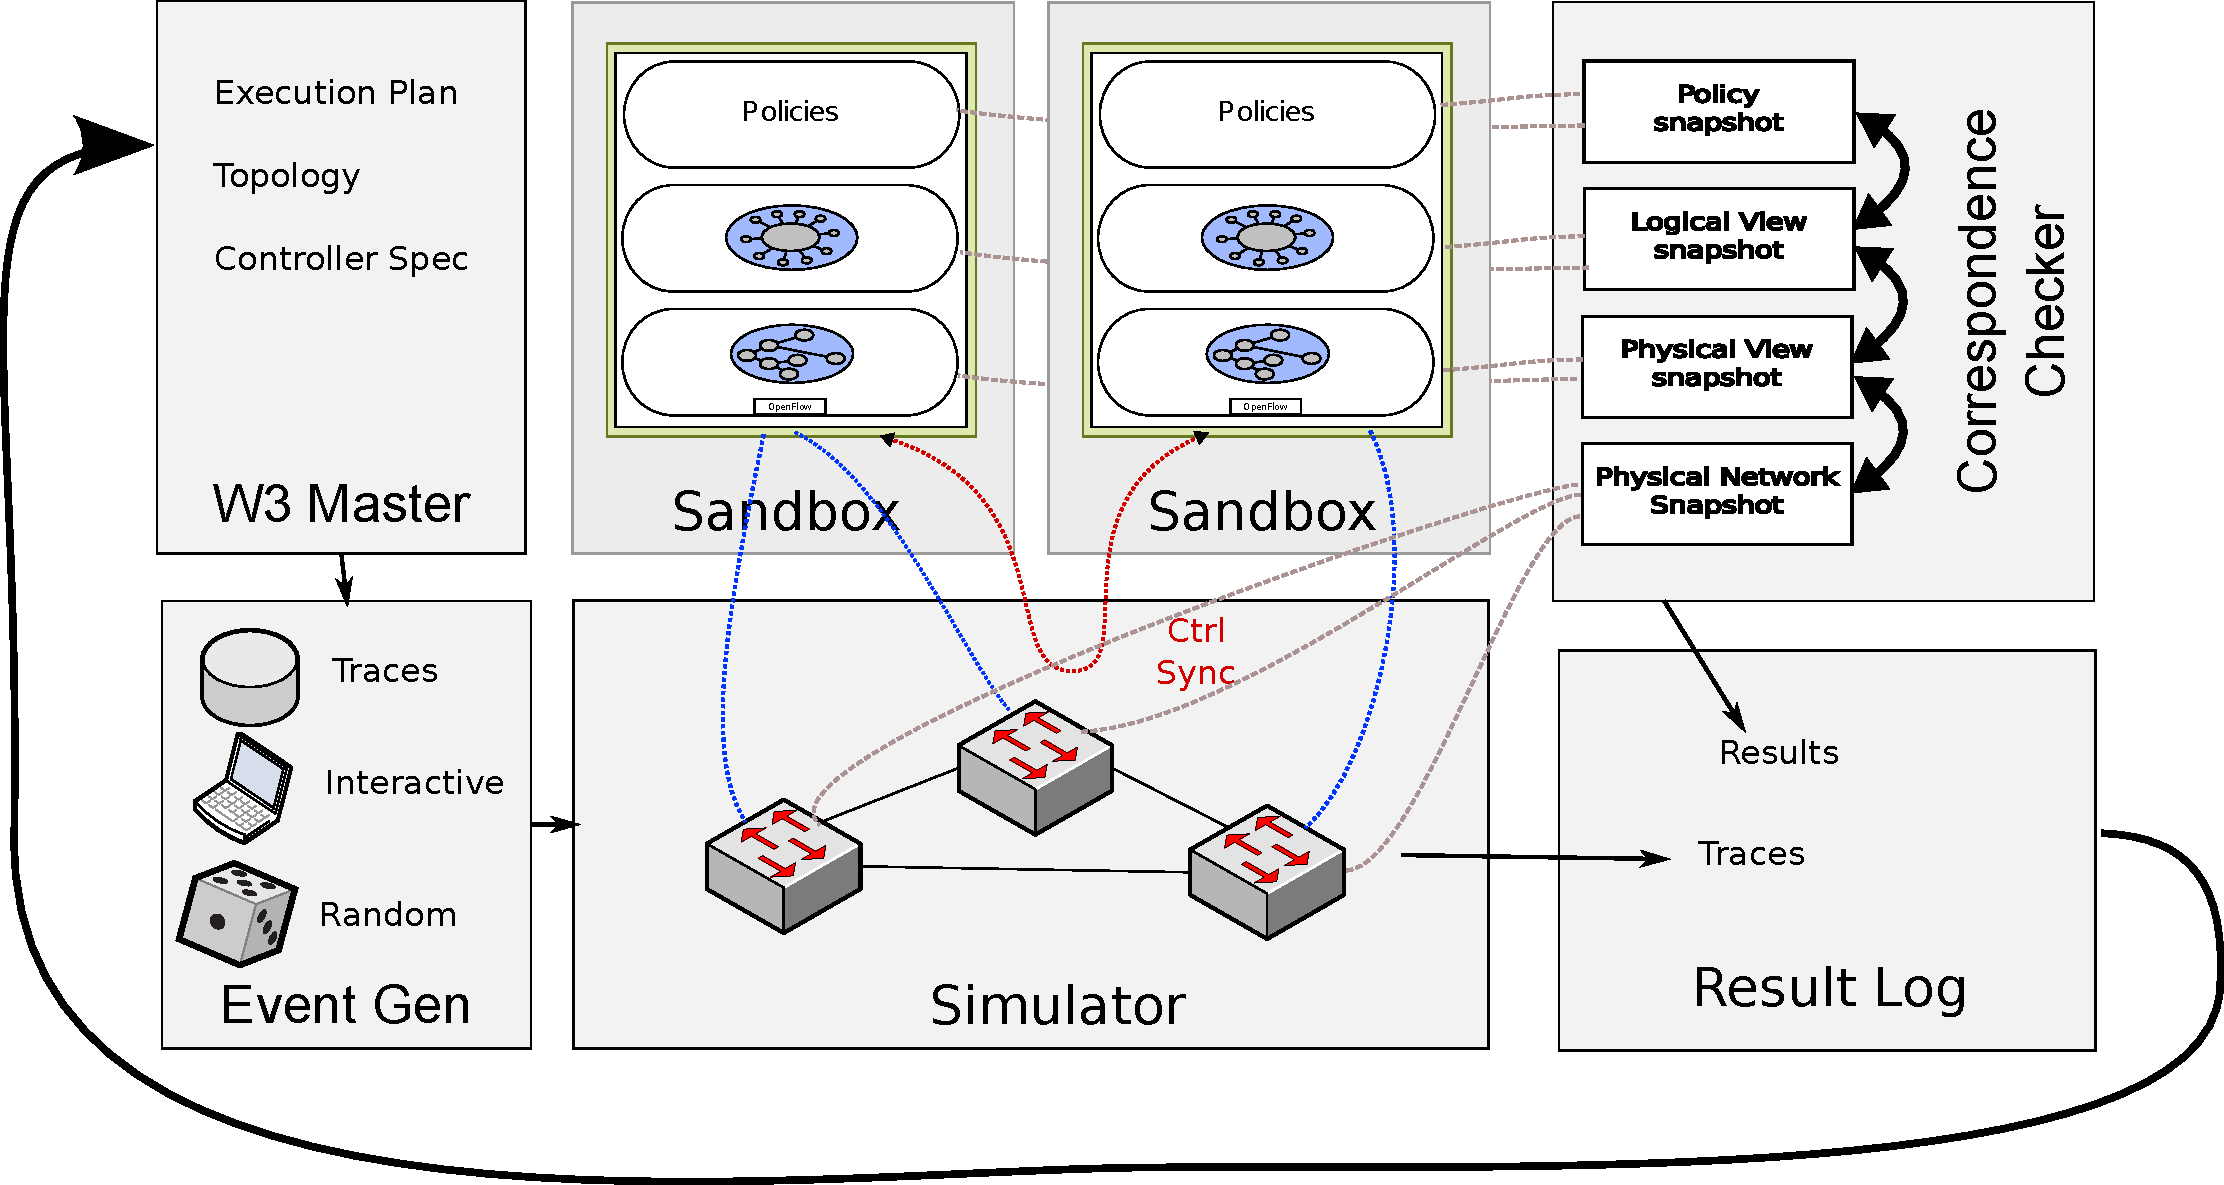
\includegraphics[width=0.8\textwidth{}]{../diagrams/architecture/architecture.pdf}
  \caption{System architecture. \colin{Andi: can haz new diagram? :P}}
  \label{fig:system}
\end{figure*}

\noindent{\bf Trace Input And Fuzzing.} Since a major goal of \projectname{} was
to support a wide range of usage scenarios, % WAT does that even mean
we provide support for three different methods for generating network trace
inputs. The most common method is to insert failure and topology change logs
from production deployments into the simulator for replay. Input traces may
also be produced synthetically with configurable, random probabilities for
network events. Lastly, we support interactive use, where the troubleshooter
has complete control over network events, and is thereby free to explore her
intuitions in order to reproduce a failure mode she has in mind.

\noindent{\bf Simulator.} We have built a simulator for SDN networks,
where network devices and hosts are modeled as lightweight python objects.
\colin{Reviewer OA: python objects creep in to the writing} Within a single thread, we
are able to deterministically model the execution of very large networks.
Our simulated model supports a wide
range of failure modes, and provides fine-grained control over event
orderings, component failures, and other aspects of the system execution. Our
simulator currently supports switch failures, link failures, arbitrary packet
re-orderings, drops and delays, and a fully general control plane.

The main challenge we encountered in the design of the simulator was
maintaining large numbers of TCP connections to the
controller(s). Although the controllers themselves may be spread
over multiple physical servers, the main simulator must nonetheless handle all
TCP connections between switches and controllers within a single process.
We ultimately ended up using epoll to avoid limitations of the UNIX select
implementation.

\noindent{\bf Controller Sandbox.} One of our major goals for \projectname{}
was to be able to run any SDN controller on top of the platform, with minimal
code changes to the controllers themselves. In addition, control servers
running on top of the simulated network must support deterministic execution
for reproducible results.

Currently we run applications as UNIX processes outside of the simulator.
We note however that there are a number of approaches for achieving deterministic
replay for external software. For example: a software determinism layer (e.g.
deterministic random number generators \colin{Reviewer OA: Whenever I see
replay, I worry about dealing with nondeterminism and pseudorandom number
generators. It was not clear how you are dealing with these issues.}) is
extremely lightweight, but requires modifications to the external software;
binary rewriting does not require any modification to the external
software's source code, but incurs moderate performance overhead; and VMs
fully support deterministic replay, but only a relatively small number of VMs can be run
on a single machine. We hope to leverage this previous work in future versions
of \projectname{}. Nonetheless, our architecture does not prevent us from
running controllers on different physical
servers in case we encounter memory or CPU bottlenecks.

\noindent{\bf Correspondence Checking.}
\projectname{} leverages the Hassel library provided by HSA~\cite{hsa}
to implement the correspondence checking algorithm. We optimize the code
slightly to run efficiently on large networks; in particular, we parallelize
symbolic packet propagation to a large number of subtasks. Correspondence
checking currently requires a small code change to the controller to fetch
the platform's view of the network state.

\projectname{} is written in roughly 10,000 lines of python, and is publicly
available. [anon]

}
